\documentclass[./main.tex]{subfiles}
%\externaldocument{/chapter1}
\begin{document}
%\tableofcontents
%\newpage

En el capítulo \ref{ch2} mostramos que la actividad pulsátil de ERK en ESCs es variable entre células (figura \ref{C2_fig:actividad}A).  En el capítulo \ref{ch3} confirmamos que esta variabilidad se mantiene estimulando a las células con dosis controladas de ligando (figura \ref{C3_fig:FGF_actividad}A), e incluso en tipos celulares más diferenciados como son las EpiSCs (figura \ref{C3_fig:EPI_activity}A). Esta heterogeneidad que observamos en la dinámica de activación de ERK en ESCs podría ser relevante para profundizar en la comprensión sobre decisiones del destino celular en las células pluripotentes. Esta observación podría ser producto de diferencias estables en el comportamiento dinámico entre las células, o podría ser que las células individuales tengan transiciones de estados oscilatorios activos e inactivos. Si estas transiciones suceden en escalas temporales largas en comparación con las mediciones, explicaría el comportamiento heterogéneo en la dinámica pulsátil que observamos.

Para evaluar estas hipótesis, en el presente capítulo estudiamos la dinámica de actividad de ERK en escalas temporales largas, comparables con el ciclo celular. Comenzamos por introducir nuevos protocolos experimentales que nos permiten adquirir la señal de actividad de ERK durante todo el ciclo celular, en donde para evitar la fototoxicidad reducimos la frecuencia de adquisición de las películas. Estas series temporales son más largas, pero de menor resolución que con las que trabajamos en los capítulos anteriores. A partir de estas características, proponemos un nuevo protocolo de detección de pulsos y análisis de estas nuevas series temporales, que luego nos permiten estudiar posibles variaciones de la dinámica de activación de ERK en escalas temporales largas. 



\section{Mediciones de la actividad dinámica de ERK a lo largo del ciclo celular}


Para evaluar posibles variaciones de escalas temporales largas de la dinámica de actividad de ERK en células madre embrionarias individuales, necesitábamos adquirir series temporales de actividad de ERK de la mayor duración posible. Para esto, nos propusimos desarrollar un diseño experimental que nos permitía registrar células durante su ciclo celular completo. El ciclo celular de las mESCs dura entre 11 y 14 horas, por lo que debíamos filmar colonias celulares durante por lo menos ese tiempo (sección \ref{C1_sec:ESC}). Además, necesitábamos conservar a las células en un medio cuya variabilidad a lo largo del tiempo de adquisición sea la menor posible. Por esta razón, decidimos medir la actividad de ERK en células de tipo \textit{wild type} que crecían en el medio N2B27. De esta manera, nos centramos exclusivamente en la actividad de ERK impulsada por la señalización de FGF4 producido por las mismas células. Entonces, evitamos estimularlas con FGF4 exógeno para prevenir su posible agotamiento, lo que aportaría variabilidad en las mediciones. Con esta misma idea, como control negativo utilizamos células que tenían una mutación de pérdida en el gen \textit{Fgf4} crecidas en el mismo medio. Como condición extra, a modo de experimento control, decidimos medir la actividad de ERK en células de tipo \textit{wild type} crecidas en s+L. Con esta condición, podríamos inferir si el estímulo endógeno y exógeno de las células tienen efectos distintos en la actividad dinámica de ERK.

Grabamos películas durante 18 horas para poder seguir células desde que nacían hasta que se dividían (figura \ref{C4_fig:experiment}A). Para reducir la exposición de las células a la luz, el tiempo entre cuadro y cuadro debía ser lo más largo posible. A efectos de nuestros objetivos, era necesario que la tasa de adquisición nos otorgue una resolución temporal que nos permita detectar la presencia de pulsos individuales, pero no hacía falta localizar los mínimos que determinan el principio y el final de un pulso. Con estas limitaciones, elegimos una frecuencia de muestreo 5 veces menor que la de los experimentos de los capítulos anteriores, y registramos un cuadro cada 105 segundos. Según el criterio de Nyquist, esta resolución temporal era suficiente para resolver pulsos de actividad de ERK con un intervalo de al menos $5.25$ minutos, lo que era adecuado para resolver pulsos con intervalos de interpulsado como los medidos previamente (figuras \ref{C2_fig:analisis_pulsos_sucesivos}B y \ref{C3_fig:FGF_consecutive}A). Logramos observar en las filmaciones una translocación repetitiva del sensor entre el citoplasma y el núcleo en el caso de células \textit{wild type}, efecto que no observamos en las mutantes.


\begin{figure}
    \centering
    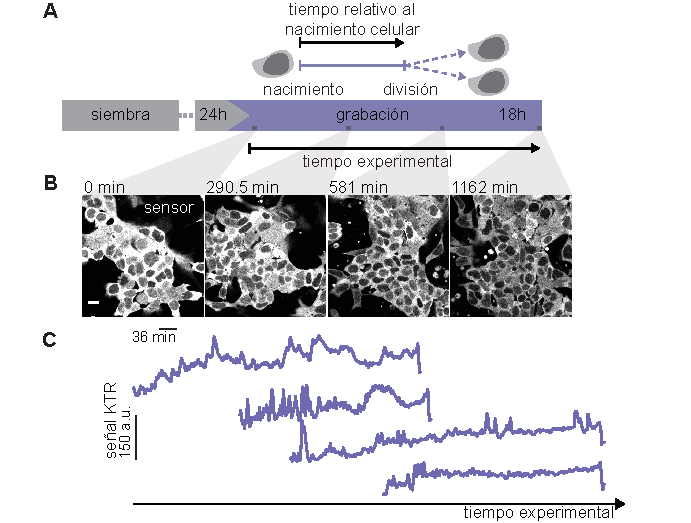
\includegraphics[width=1\columnwidth]{figures/chapter4/C4_experiment.pdf}
    \caption{\textbf{Mediciones de la actividad de ERK que abarcan todo el ciclo celular.} (A) Esquema del protocolo experimental para registrar los picos de ERK a lo largo del ciclo celular completo. (B) Fotomontaje de una colonia de ESCs que expresa el sensor KTR en el curso de un experimento. Barra de escala: 20 $\mu$m. (C) Ejemplos de series temporales de la señal KTR obtenidos como la intensidad media de una ROI nuclear medida en la imagen invertida en células de tipo \textit{wild type} que crecen en N2B27. La tasa de adquisición fue de 105 s/cuadro. Las mediciones comienzan inmediatamente después de un evento de división celular y se grafican en relación con el tiempo experimental absoluto. Los detalles del experimento se encuentran en \cite{Fabris2022}.}
    \label{C4_fig:experiment}
\end{figure}

Para obtener series temporales de la dinámica de actividad de ERK, medimos la intensidad media de la fluorescencia invertida del sensor KTR en una región de interés de área variable en el núcleo (figuras \ref{C4_fig:experiment}C y \ref{C4_fig:traces}). Comenzamos el \textit{tracking} de una célula individual el cuadro posterior a la división celular en donde era posible seguir a la célula, y lo terminamos cuando la célula que seguíamos se dividía. Conservamos en el análisis los \textit{trackings} de las células que abandonaban nuestro campo de visión solamente si las habíamos seguido durante al menos más de $4.5$ horas. Por otro lado, la mayoría de las mediciones terminaban con la exclusión del sensor del núcleo antes de la división celular, lo que se traducía en un pico de alta amplitud al final en cada traza (figura \ref{C4_fig:experiment}C). Dado que este pico no era informativo sobre la dinámica de actividad de ERK, lo recortamos antes de implementar cualquier estrategia de análisis sobre las series temporales. 

Observamos en la figura \ref{C4_fig:experiment}B que, en promedio, la señal del sensor de traslocación KTR aumentaba a medida que pasaba el tiempo. Esto reflejaba una disminución general de los niveles de fluorescencia del sensor KTR en estas mediciones largas. Al ser estas mediciones $12.5$ veces más largas que las adquiridas en los capítulos anteriores, el ruido de baja frecuencia era más significativo. Este efecto inevitablemente se trasladó a las series temporales de la figura \ref{C4_fig:traces}. 

Las series temporales mostraban una dinámica pulsátil en el caso de células \textit{wild type}, pero no en las mutantes (figuras \ref{C4_fig:experiment}C y \ref{C4_fig:traces}). Sin embargo, presentaron diferencias cualitativas respecto a las series temporales de los capítulos anteriores. Por un lado, su resolución estaba elegida para localizar pulsos en la serie temporal, pero no analizar su forma. Por otro lado, el ruido se veía distinto en este caso, y en particular el ruido en bajas frecuencias era más importante que en las señales de alta resolución temporal. Estas características requirieron elaborar un nuevo protocolo de detección de pulsos y una nueva estrategia de análisis de datos. 


\begin{figure}
    \centering
    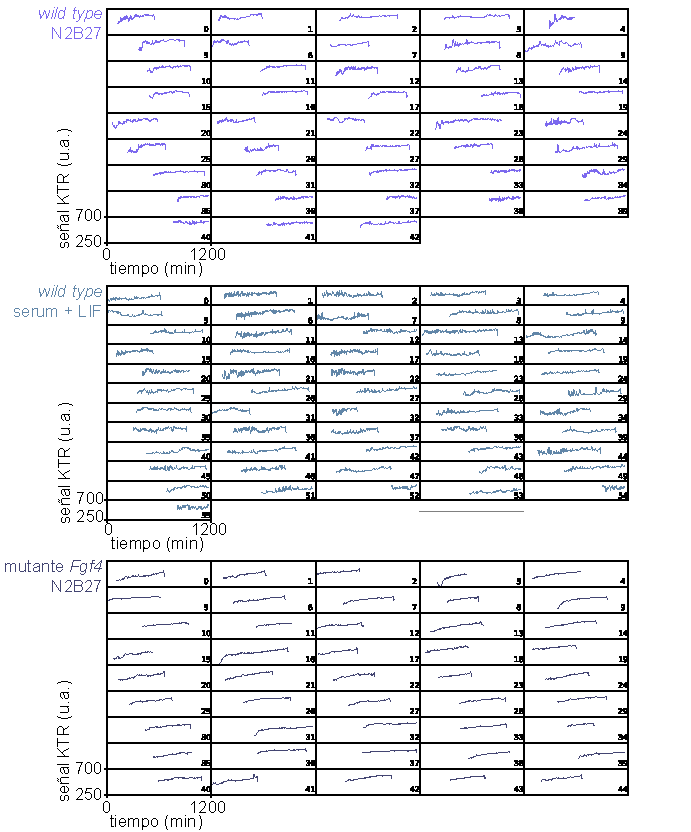
\includegraphics[width=1\columnwidth]{figures/chapter4/C4_traces.pdf}
    \caption{\textbf{Series temporales de la señal KTR de larga duración.} Series temporales de la señal KTR obtenidos como la intensidad media de una ROI nuclear medida en la imagen invertida en células de tipo \textit{wild type} que crecen en N2B27 (arriba), serum + LIF (centro), y en células mutantes \textit{Fgf4} que crecen en N2B27 (abajo). La tasa de adquisición fue de 105 s/cuadro. Las mediciones comienzan inmediatamente después de un evento de división celular y se grafican en relación con el tiempo experimental absoluto. Los detalles de la medición se encuentran en \cite{Fabris2022}.}
    \label{C4_fig:traces}
\end{figure}

\section{Detección de pulsos de actividad en series temporales de larga duración}
\sectionmark{Detección de pulsos}
\label{C4_sec:pulse_detection}

En la detección de pulsos de las series temporales como las de la figura \ref{C4_fig:experiment}C, nos centramos exclusivamente en su localización en las series temporales. En consecuencia, necesitábamos solamente identificar los máximos, o picos, de los pulsos de actividad de ERK. Para llevar a cabo esta tarea, primero filtramos las bajas y altas frecuencias, y luego establecimos un enfoque que permitiera distinguir los picos sobre el ruido en estas series temporales con una resolución temporal considerablemente más baja que las analizadas previamente. 

Las series temporales presentaban fluctuaciones de baja y alta frecuencia. El ruido de baja frecuencia creaba tendencias variables que impedían la comparación directa entre series temporales. El ruido de alta frecuencia podría dificultar la identificación de los pulsos de actividad. Para asegurarnos de filtrar el ruido y perder la menor cantidad posible de información sobre la dinámica de actividad de ERK, empleamos dos estrategias de filtrado diferentes. Estas dos estrategias generaron dos conjuntos de datos que analizamos por separado. Favorablemente, ambas estrategias produjeron estadísticas similares tras la detección de picos. Los filtrados consistían en (i) restar la línea de base que solamente filtraba las frecuencias bajas, y (ii) un filtro de pasa banda que eliminaba tanto las frecuencias bajas como las altas \ref{C4_fig:pulse_detection}. 


\begin{figure}
    \centering
    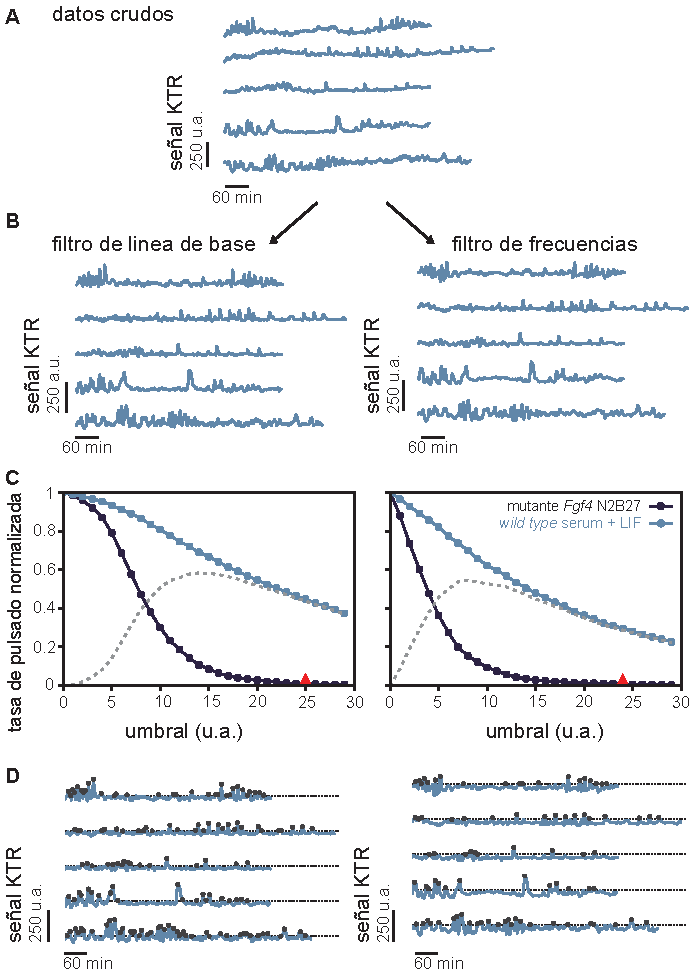
\includegraphics[width=1\columnwidth]{figures/chapter4/C4_pulse_detection.pdf}
    \caption{\textbf{Detección de picos y análisis de umbrales en series temporales de larga duración.} (A) Series temporales representativas de la señal KTR de películas de largo plazo en células individuales de tipo \textit{wild type} que crecen en serum + LIF. Las series temporales se han alineado en relación con el momento del nacimiento de la célula para esta ilustración. (B) Las mismas series temporales que en A tras el filtrado. (C) Gráfico de la frecuencia de pulsado total normalizada en función del umbral de la señal KTR filtrada para explorar cómo el número de pulsos detectados depende del valor del umbral. Células mutantes \textit{Fgf4} creciendo en N2B27 en azul, células de tipo \textit{wild type} creciendo en serum + LIF en celeste. La línea punteada gris representa la diferencia de las frecuencias de pulsado total normalizadas entre las condiciones experimentales consideradas. La posición del valor umbral de intensidad seleccionado $I_{\text{th}}$ está marcada con un triángulo rojo. (D) Las mismas series temporales que en B con los picos identificados (puntos negros). La línea gris punteada indica el parámetro umbral seleccionado $I_{\text{th}}$. (B-D) Se ilustran las dos estrategias de filtrado, la columna de la izquierda corresponde al filtrado de línea base y la de la derecha al filtrado en frecuencias.}
    \label{C4_fig:pulse_detection}
\end{figure}


En la primer estrategia, que llamamos \textbf{filtro de linea\\de base}, restamos un polinomio de grado bajo a las series temporales (figura \ref{C4_fig:pulse_detection}B).\marginpar{filtro de linea de base} Para obtener este polinomio, primero detectamos todos los mínimos locales de cada serie temporal. Comparamos cada punto $x_i$ de la serie temporal con sus dos vecinos más cercanos $x_{i-2},x_{i-1}, \text{ y } x_{i+1},x_{i+1}$. El valor $x_1$ se comparó con sus dos vecinos a la derecha y con su único vecino $x_0$ a la izquierda, y $x_{n-2}$ con sus dos vecinos a la izquierda y con su único vecino $x_{n-1}$ a la derecha. Utilizamos cuadrados mínimos para ajustar un polinomio a los mínimos detectados, y a los puntos del borde de la serie temporal $x_0$ y $x_{n-1}$ \cite{Harris2020}. Debido a que las series temporales tenían duraciones distintas, establecimos el grado del polinomio como $\text{deg}_j = (2+m_j) / 3$, donde $m_j$ es el número de mínimos detectados para la serie temporal $j$. De esta manera buscamos ajustar la línea de base de cada serie temporal, y evitar el sobreajuste que conduciría a restar parte de la señal a la serie temporal.  



En la segunda estrategia, que llamamos \textbf{filtro de frecuencias}, eliminamos de las series temporales las frecuencias altas y bajas no deseadas con un filtro de pasa banda (figura \ref{C4_fig:pulse_detection}B)\marginpar{filtro de frecuencias}. Aplicamos un filtro Butterworth, que es un filtro cuadrado de pasa banda: tiene una respuesta de frecuencia plana en la región de la banda de paso, y se reduce a cero en la región de la banda de parada \cite{Butterworth1930}. Su orden regula la nitidez del corte y nosotros lo fijamos en 4. Además, lo implementamos en una ventana temporal móvil tanto hacia adelante como hacia atrás en el tiempo, de modo que el filtro tenía tiempo cero y fase lineal (submódulo scipy Signal \cite{Virtanen2020}). Utilizamos una extensión impar de 15 cuadros para la señal, es decir, 3 veces el número de coeficientes de los polinomios de Butterworth. Elegimos las frecuencias de corte $f_{\text{low}}$ y $f_{\text{high}}$ en función de la frecuencia de Nyquist, tal que $f_{\text{low}}= 0,025 \times f_{\text{nyq}}$ y $f_{\text{high}}=0,6 f_{\text{nyq}}$, con $f_{\text{nyq}}=0,5 f_s =(1/210) $Hz para una frecuencia de muestreo $f_s=(1/105) $Hz.    



Una vez aplicados los filtros, determinamos los máximos locales comparando valores vecinos. Es decir, comparamos cada valor $x_i$ de la serie temporal con sus vecinos $[x_{i-\delta}, x_{i-1}]$ y $[x_{i+1}, x_{i+\delta}]$, donde $\delta$ es un parámetro libre del método que determina el intervalo de tiempo mínimo entre picos que podríamos resolver. En los bordes de las series temporales, redujimos el rango de comparación hasta alcanzar $[x_1, x_\delta]$ para el valor inicial $x_0$, y $[x_{n-\delta}, x_{n-2}]$ para el valor final $x_{n-1}$. Motivados por las mediciones realizadas en los capítulos anteriores sobre series temporales de mayor resolución, fijamos $\delta = 2$ cuadros, lo que nos permitió resolver los picos de actividad de ERK que están separados por al menos $5.25$ minutos.


Para eliminar los picos espurios de baja amplitud, los filtramos con un valor umbral $I_{\text{th}}$ de señal KTR. Para esto, exploramos cómo cambiaba el número de picos en las células mutantes de \textit{Fgf4} en N2B27 (control negativo, donde no se esperan picos) y en las células de tipo \textit{wild type} que crecían en s+L (control positivo, donde se esperan más picos) a medida que cambiábamos este umbral (figura \ref{C4_fig:pulse_detection}C). Detectamos picos en las dos condiciones para diferentes valores de umbral de $I_{\text{th}}^i$ espaciados uniformemente en el rango $[0, 30] $u.a. Para cada $I_{\text{th}}^i$, calculamos la \textbf{frecuencia de pulsado total} como
\marginpar{frecuencia de\\pulsado total}
\begin{equation}
    \delta^i = \sum_{j=1}^N \frac{n_j^i}{L_j},
\end{equation}
donde $N$ es el número total de células de cada condición, $n_j^i$ es el número de pulsos detectados para este valor umbral $I_{\text{th}}^i$ y $L_j$ es la duración de la serie temporal de la célula $j$. Luego, para poder comparar esta cantidad entre condiciones, la normalizamos por la frecuencia de pulsado total $\delta_0$ calculada cuando $I_{\text{th}}^0=0$, definiendo la \textbf{frecuencia de pulsado total normalizada} como \marginpar{frecuencia de\\pulsado total\\normalizada}
\begin{equation}
     \overline{\delta_i} =  \delta^i / \delta^0.
\end{equation}
Observamos que esta cantidad disminuía con el aumento de los valores del umbral tanto en el control negativo como en el \textit{wild type} (figura \ref{C4_fig:pulse_detection}C). En el caso del control negativo, la frecuencia de pulsado total normalizada decaía mucho más rápidamente, llegando a $0.5$ mientras que los valores del \textit{wild type} seguían siendo alrededor de $0.9$. A partir de esta observación, inferimos que existían valores de umbrales que permitían distinguir picos de actividad presentes en las series temporales de \textit{wild type} de las fluctuaciones presentes el control. Establecimos un valor umbral $I_{\text{th}}$ para el que el $1 \%$ de todos los máximos locales se clasificaran como picos en el control negativo, es decir, $\overline{\delta^i}=0,01$. Esta condición resulta en valores de umbral $I_{\text{th}}=24$ para la estrategia de filtrado de frecuencia e $I_{\text{th}}$=25 para la estrategia de filtrado de linea de base (figura \ref{C4_fig:pulse_detection}D). A continuación presentaremos el análisis que surgió de la estrategia de filtrado (i) de linea de base, y el que surgió de la otra estrategia de filtrado se puede ver en el apéndice \ref{C4_ap:band_pass_filter_cell_cycle}. Como control, graficamos la distribución de intervalos de interpulsado en la figura \ref{C4_fig:IPI}. En este conjunto de datos, la distribución del IPI fue consistente con los obtenidos con mayor resolución temporal de las figuras \ref{C2_fig:analisis_pulsos_sucesivos}B y \ref{C3_fig:FGF_consecutive}A. 

\begin{figure}
    \centering
    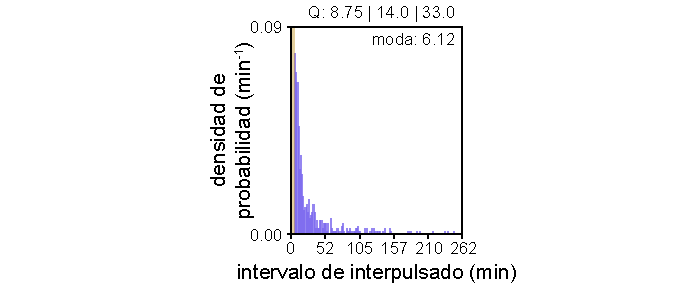
\includegraphics[width=1\columnwidth]{figures/chapter4/C4_IPI.pdf}
    \caption{\textbf{Distribución de intervalos de interpulsado para las mediciones de larga duración.} Las series temporales fueron filtradas con el filtro de linea de base. Se indican el límite de resolución del algoritmo de detección de pulsos (barra amarilla) y los cuartiles (Q) 25, 50 y 75.}
    \label{C4_fig:IPI}
\end{figure}


Presentamos el resultado de la detección de pulsos en \textit{raster plots}, donde es posible visualizar la localización de los pulsos en cada serie temporal que adquirimos (figura \ref{C4_fig:raster_plot}). Como primera impresión, notamos que los pulsos se concentraban hacia el principio del ciclo celular. Esta observación podría ser efecto de posibles variaciones de escalas de tiempos largos en la actividad pulsátil de ERK. Además, podrían existir condiciones experimentales no estacionarias, como las que observamos en figuras \ref{C4_fig:experiment}B y C, y \ref{C4_fig:traces}, que contribuyan a esta variabilidad.


\begin{figure}
    \centering
    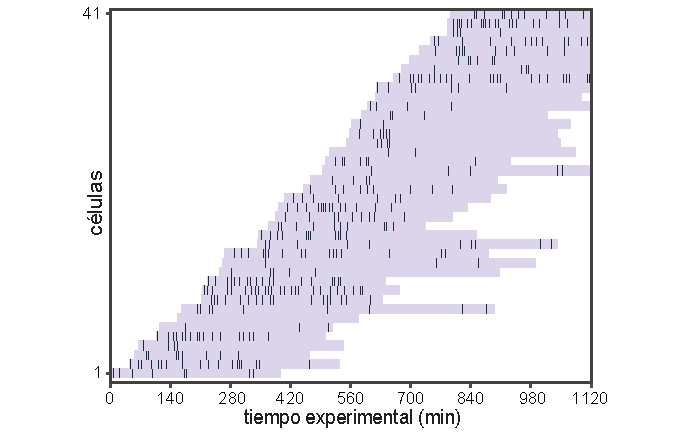
\includegraphics[width=1\columnwidth]{figures/chapter4/C4_raster_plot.pdf}\caption{\textbf{La localización de los pulsos se concentra al principio del ciclo celular, y depende del tiempo experimental absoluto.} \textit{Raster plot} que muestra la localización de los pulsos de actividad de ERK a lo largo del ciclo celular. Las bandas horizontales de color violeta se extienden desde el nacimiento hasta la división de células individuales, las barras verticales oscuras representan los picos de los pulsos. Las trazas de las células individuales comienzan inmediatamente después de la división celular y se representan en relación con el tiempo experimental absoluto. }
    \label{C4_fig:raster_plot}
\end{figure}

\section{Mediciones relativas al ciclo celular}
\label{C4_sec:analisis}

Para distinguir si nuestra observación de mayor cantidad de pulsos al principio del ciclo celular era producto de posibles variaciones de escalas de tiempos largos en la actividad pulsátil de ERK o de posibles condiciones experimentales no estacionarias, era necesario encontrar la manera de visualizar cada una de estas contribuciones por separado. Para esto, introdujimos un mapa temporal bidimensional, en donde las coordenadas en este mapa son el tiempo $T_e$ experimental medido desde el comienzo de la filmación y el tiempo $T_b$ relativo al nacimiento de la célula individual. Para cada célula $i$, su representación comienza en $T_b^i= 0$ y $T_e^i$ en el tiempo en que nació la célula $i$ medido desde el inicio del registro. Desde este punto del mapa, las series temporales individuales se representarían a lo largo de una línea diagonal de pendiente unidad. Para estudiar el comportamiento de la población y evitar la superposición de series temporales individuales en el mapa, trazamos la \textbf{frecuencia de pulsado promediada} \marginpar{frecuencia de\\pulsado\\promediada}en intervalos de $70$ minutos a lo largo de ambos ejes. En cada intervalo, contamos el número total de pulsos de todas las trazas en ese intervalo y lo dividimos por el número total de minutos de grabación que contribuyen. En este mapa de frecuencia de pulsado, los efectos del ciclo celular se manifestarían como un cambio de frecuencia en la dirección horizontal (figura \ref{C4_fig:cell_cycle_effect}A, panel superior), mientras que las condiciones experimentales no estacionarias se manifestarían como un cambio de frecuencia en la dirección vertical (figura \ref{C4_fig:cell_cycle_effect}A, panel inferior). En la figura \ref{C4_fig:cell_cycle_effect}B podemos observar que los valores de frecuencia de pulsado disminuían de derecha a izquierda. Esto indica que la actividad pulsátil decae a lo largo del ciclo celular. Sin embargo, la frecuencia de pulsado también disminuía desde la parte inferior hacia la superior, mostrando simultáneamente efectos relacionados a las condiciones experimentales no estacionarias. 


\begin{figure}
    \centering
    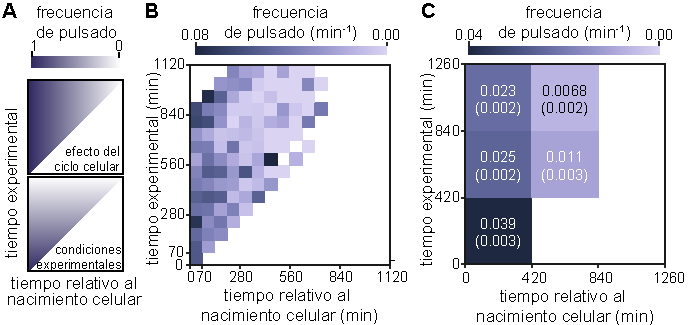
\includegraphics[width=1\columnwidth]{figures/chapter4/C4_cell_cycle.pdf}\caption{\textbf{Los pulsos de ERK son más frecuentes al comienzo del ciclo celular.} (A) Esquema de las expectativas de una reducción de la actividad pulsátil debida al ciclo celular (arriba) y a la modificación de las condiciones experimentales (abajo) en el mapa bidimensional de frecuencias de pulsado promediada codificado en color. (B) Mapa de frecuencia de pulsado promediada para los datos mostrados en la figura \ref{C4_fig:raster_plot}. El tiempo está discretizado en intervalos de 70 minutos. (C) Mapa de frecuencia de menor resolución que muestra la frecuencia de pulsado media y su error estimado entre paréntesis. El tiempo está discretizado en intervalos de 420 minutos.}
    \label{C4_fig:cell_cycle_effect}
\end{figure}



Para cuantificar esta observación, discretizamos este mapa temporal bidimensional en cuadrados más grandes, que representan intervalos de tiempo mayores (figura \ref{C4_fig:cell_cycle_effect}C). Calcular la frecuencia de pulsado en cada cuadrado fue desafiante, pues no siempre todas las series temporales abarcaban el intervalo de tiempo completo. Para introducir cómo implementamos esta cuantificación, nos vamos a focalizar primero en calcular la frecuencia de pulsado para una sola serie temporal en un dado intervalo de tiempo, en donde el tiempo es discreto $t_i$, siendo $i \in [0,f]$. Podemos pensar que en cada instante $t_i$ del intervalo de tiempo considerado, la serie temporal en ese instante representa un experimento individual con dos posibles resultados: 1 (éxito - si la célula pulsa en ese instante) y 0 (fracaso - si no pulsa). Además, la probabilidad de pulsar de la célula en ese instante de tiempo es $p \in [0,1]$. Extendiendo esta idea, podemos pensar que cada célula en cada instante del intervalo de tiempo entre $t_0$ y $t_f$ es un experimento independiente, siendo un total de $T$  experimentos. Entonces, la probabilidad de obtener $r$ números de éxito (o pulsos) en los $T$ experimentos independientes está determinada por la distribución binomial $B(r;T,p)$. Nos interesa estimar el número relativo de éxitos en $T$ ensayos $\overline{\hat{r}}= \hat{r}/T$, es decir, la frecuencia de pulsado en ese intervalo de tiempo. Entonces, el estimador de máxima verosimilitud para $\hat{r}$ viene dado por $\overline{\hat{r}}= r/T$ y su varianza $\sigma^2 =  r (1-r)/T$ \cite{Frodesen1979}. En este caso, $r$ es el número de pulsos detectados en el intervalo de tiempo considerado en todas las células que contribuyen, y $T$ es la suma de las duraciones de las series temporales en el intervalo de tiempo considerado. Con este criterio, estimamos la frecuencia de pulsado promediada en intervalos de tiempo de $420$ minutos, que representamos en un mapa bidimensional en donde sus coordenadas eran el tiempo medido desde el comienzo de la filmación y el tiempo relativo al nacimiento de la célula individual (figuras \ref{C4_fig:cell_cycle_effect}C). Calculamos el error de esta cantidad como su desviación estándar. En esta aproximación asumimos condiciones estacionarias para intervalo de tiempo de 420 minutos a través de considerar $p$ constante en cada caso. Despreciamos pequeñas variaciones en $p$ porque queríamos estudiar el comportamiento de la actividad dinámica de escalas temporales cortas previamente caracterizada (aprox. 7 min) en escalas de tiempo largas (aprox. 13 horas). 


En esta cuantificación, observando el comportamiento de abajo hacia arriba podemos ver que la frecuencia de pulsado cambia a medida que aumenta el tiempo experimental, posiblemente producto de efectos relacionados a las condiciones experimentales no estacionarias (figura \ref{C4_fig:cell_cycle_effect}C). Por otro lado, observando el comportamiento de izquierda a derecha podemos ver que la frecuencia de pulsado era consistentemente más alta en las células que se encontraban al inicio de su ciclo celular. Obtuvimos resultados similares cuando aplicamos una estrategia alternativa de filtrado (figura \ref{C4_fig:band_pass_filter_cell_cycle}, apéndice \ref{C4_ap:band_pass_filter_cell_cycle}) y cuando analizamos a las células que crecían en s+L (figura \ref{C4_fig:s+L_cell_cycle}, apéndice \ref{C4_ap:s+L_cell_cycle}). En conjunto, estos resultados sugieren que las células son más propensas a pulsar en una fase más temprana de su ciclo celular, indicando que la actividad pulsátil de ERK tiene variaciones de escalas de tiempos largos.




\section{Conclusiones y discusión}


% PARA SISTEMAS EXCITABLES, VER https://bibliotecadigital.exactas.uba.ar/download/tesis/tesis_n3479_Eguia.pdf

En este capítulo nos preguntamos si la heterogeneidad en la actividad pulsátil de ERK que observamos en los capítulos anteriores es producto de diferencias estables en el comportamiento dinámico entre las células, o de que las células individuales tengan transiciones en escalas temporales largas en comparación con las mediciones de estados oscilatorios activos e inactivos. Para evaluar estas hipótesis, estudiamos la dinámica de actividad de ERK en escalas temporales largas, comparables con el ciclo celular. 

Adquirimos series temporales de la dinámica de actividad de ERK en células madre embrionarias de tipo \textit{wild type} durante su ciclo celular completo, donde la actividad de ERK era principalmente desencadenada por la señalización de FGF4 producido por las mismas células (figuras \ref{C4_fig:experiment}, \ref{C4_fig:traces}). Las series temporales mostraban una dinámica pulsátil, que desaparecía en células mutantes. Elaboramos un nuevo protocolo de detección de pulsos con el que fue posible localizar sus picos en las series temporales (figuras \ref{C4_fig:pulse_detection},\ref{C4_fig:raster_plot}). 
A partir del resultado de este algoritmo, observamos que los pulsos se concentraban hacia el principio del ciclo celular (figura \ref{C4_fig:cell_cycle_effect}). Esta observación podría ser efecto de posibles variaciones de escalas de tiempos largos en la actividad pulsátil de ERK, o podrían existir condiciones experimentales no estacionarias que contribuyan a esta variabilidad.

Para distinguir entre estas dos posibilidades, construimos un mapa para visualizar simultáneamente cómo cambiaba la frecuencia de pulsado del tiempo experimental y del tiempo relativo al ciclo celular. A partir de visualizar y cuantificar estos comportamientos, observamos que la frecuencia de pulsado decaía a lo largo del ciclo celular. En simultáneo, observamos que decaía con el tiempo experimental, posiblemente producto de efectos relacionados a condiciones experimentales no estacionarias. Obtuvimos resultados similares cuando aplicamos una estrategia alternativa de filtrado (figura \ref{C4_fig:band_pass_filter_cell_cycle}) y cuando analizamos a las células que crecían en s+L donde hay también estimulación exógena de FGF4 (figura \ref{C4_fig:s+L_cell_cycle}). En conjunto, estos resultados sugieren que las células son más propensas a pulsar en una fase más temprana de su ciclo celular, indicando que la actividad pulsátil de ERK tiene variaciones de escalas de tiempos largos.


El decaimiento de la actividad pulsátil de ERK a lo largo del ciclo celular puede interpretarse como una transición de las células del estado con oscilaciones a uno no oscilatorio, posiblemente a través de cambios en la relación entre la superficie y el volumen celulares que se dan a lo largo del ciclo celular, o en la expresión dependiente del ciclo celular de los componentes del sistema de señalización FGF/ERK. Sin embargo, creemos que nuestras observaciones no son suficientes para explicar el origen de la heterogeneidad en la actividad pulsátil de ERK, que parecen ser también producto de diferencias estables en el comportamiento dinámico entre las células. 

Esta interpretación introduce una posible fuente de heterogeneidad celular que podría ser relevante para las decisiones del destino celular en ESCs. En el embrión, la señalización FGF/ERK regula la diferenciación hacia el endodermo primitivo y las células del epiblasto. Diferentes actividades dinámicas de señalización pueden subyacer al establecimiento de estos dos linajes discretos a partir de un tipo celular precursor común en respuesta a la misma señal \cite{Pokrass2020}. Por otro lado, la dinámica de señalización heterogénea que describimos en los cultivos de ESCs añade otra dimensión a la variabilidad transcripcional que anticipa la diferenciación celular \cite{Canham2010,Chambers2007,Hayashi2008,Singh2007,Toyooka2008}. Aunque la señalización no está necesariamente desactivada cuando ERK no pulsa, las oscilaciones intermitentes de ERK en ESCs se parecen a la dinámica transcripcional de muchos genes, para los que se alternan ráfagas de expresión y periodos de silencio \cite{Tunnacliffe2020}. Para evaluar esta hipótesis, será en el futuro necesario correlacionar la dinámica de señalización de ERK con los programas transcripcionales del desarrollo para entender cómo se interrelacionan estos dos niveles y cómo se relacionan con la diferenciación celular.

 
\end{document}
